\pagestyle{fancy}
\renewcommand{\theUnit}{7}
\ifthenelse{\isundefined{\UnitPageNumbers}}{}{\setcounter{page}{1}}
\rhead{Chapter  \theUnit: Confidence Intervals}
\lhead{Math 3382: Statistical Theory}
%\lhead{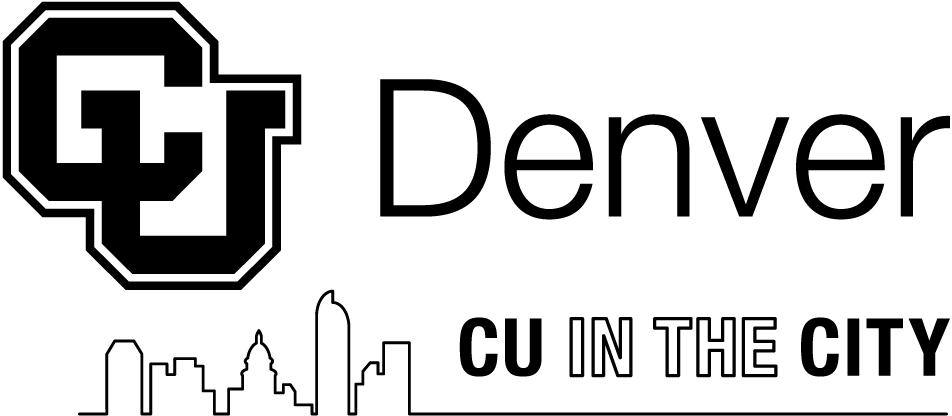
\includegraphics[width=1.25cm]{CUDenver-Logo.png}}
\rfoot{\mypage}
\cfoot{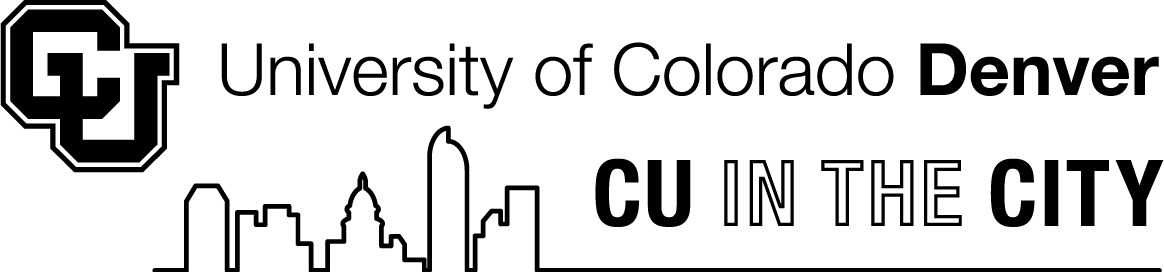
\includegraphics[width=2.25cm]{CUDenver-Logo-coverpage.png}}
\lfoot{Adam Spiegler}
\fancypagestyle{firstfooter}{\footskip = 50pt}
\renewcommand{\footrulewidth}{.4pt}
%%%%%%%%%%%%%%%%%%%%%%%%%%%
\vspace*{-20pt} \thispagestyle{firstfooter}


%\begin{tasks}[counter-format = {(tsk[a])},label-offset = {0.8em},label-format = {\color{black}\bfseries}](2)

\pagebegin{Section 7.4: Confidence Intervals for Proportions}

A recent PBS NewsHour/NPR/Marist poll\footnote{``Politics still drives how Americans fell about COVID response, one year in'', PBS, March 11, 2021} surveyed $1,\!082$ randomly selected registered voters in the US to gage their opinions on how the US is handling the COVID pandemic.

\begin{center}
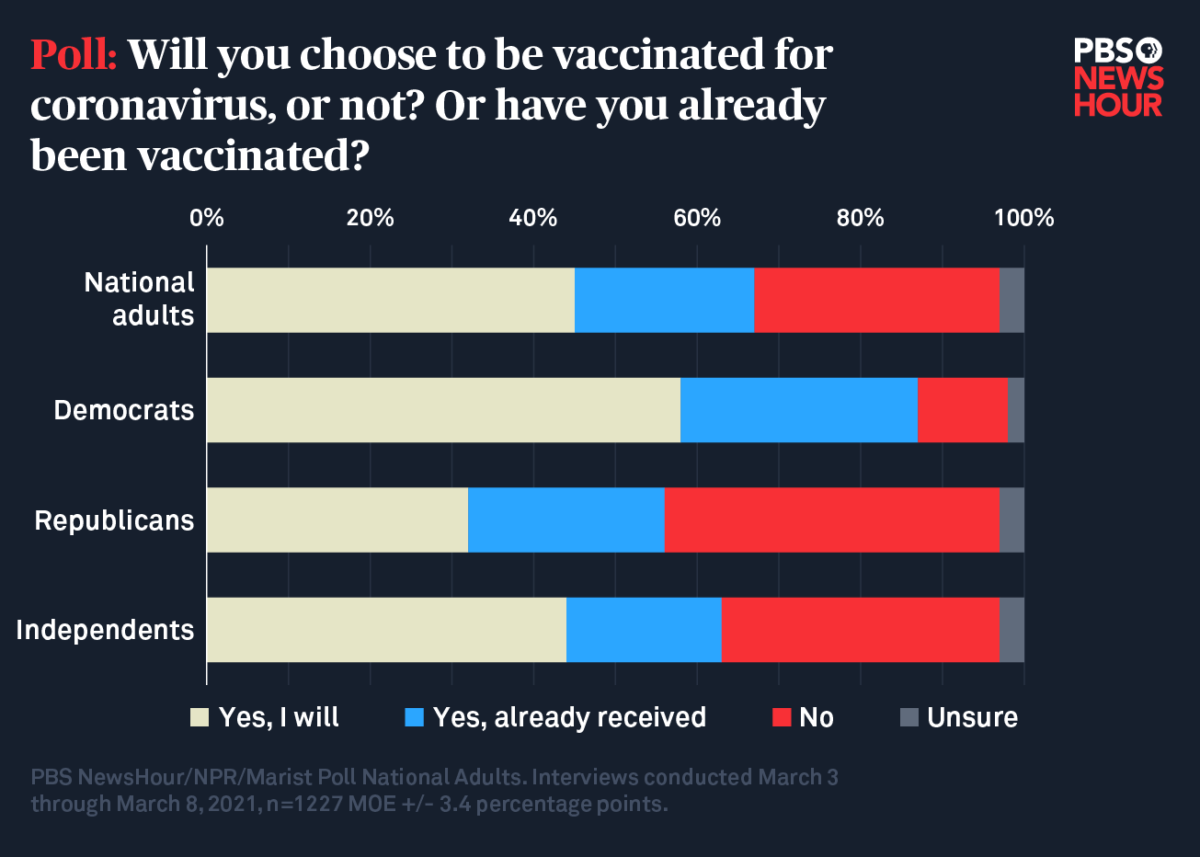
\includegraphics[width=4in]{17/vaccination-poll1.png}
\end{center}

\textbf{\colorb{Based on this survey, approximately what proportion of adults in the US do NOT plan to get vaccinated?}}

\bs

\begin{center}
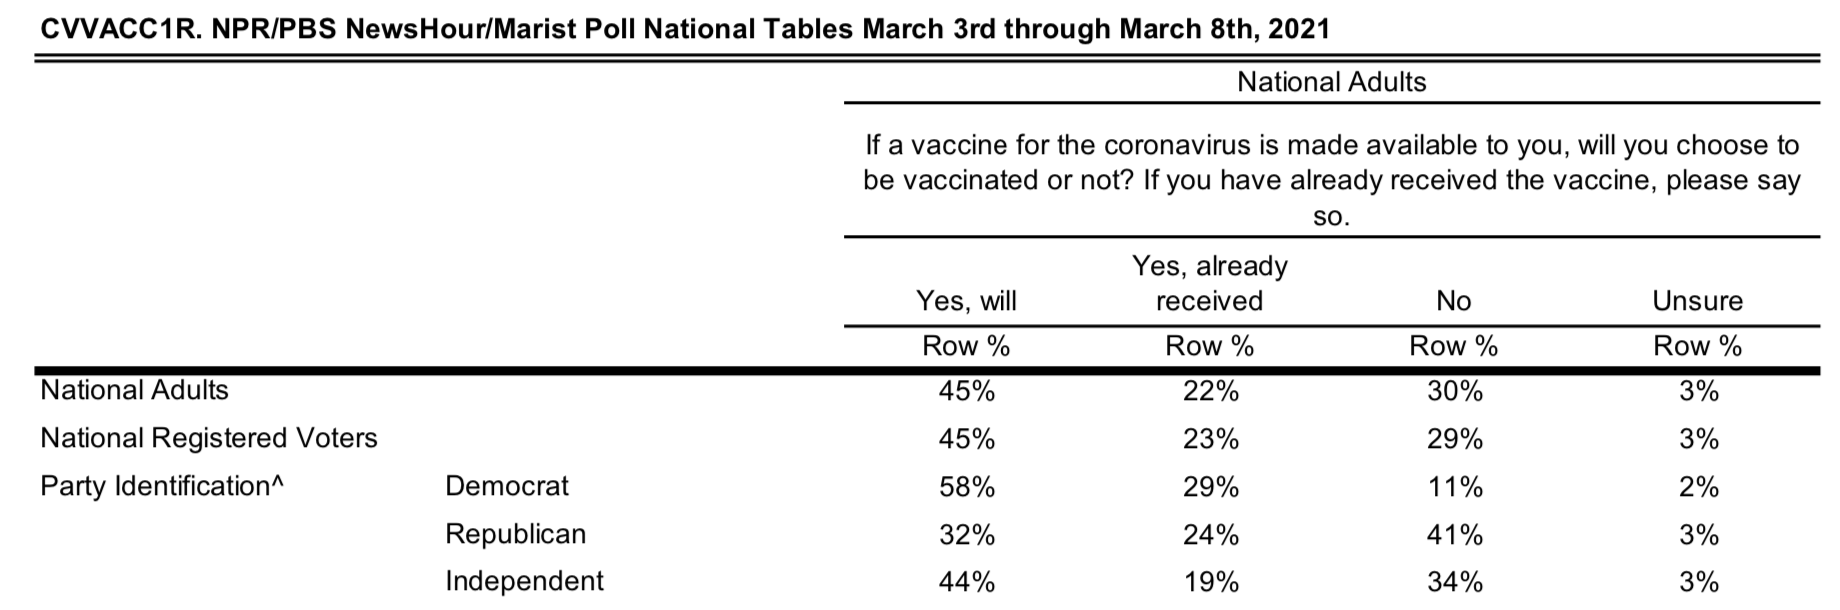
\includegraphics[width=0.95\tw]{17/vaccination-table1.png}
\end{center}

\clearpage

\bbox
Recall if $p$ is the proportion of a population that have a certain characteristic, then the distribution of the sample proportion (when samples size $n$ are randomly selected) will be
\[ \hat{p} \sim N \left( p, \sqrt{ \frac{p(1-p)}{n}} \right) \]
provided both $np \geq 10$ and $n(1-p) \geq 10$.
\ebox


\bb
\ii If we standardize the distribution for the sample proportion we have
\[ P \left( -1.96 < Z < 1.96 \right) = P \left( -1.96 < \frac{p - \hat{p}}{\sqrt{(p(1-p))/n}} < 1.96 \right).\]
Give an interval which will contain the value of $p$ 95\% of the time.\label{rough-approx}


\vfill

\ii Construct a 95\% confidence interval to estimate the proportion of all adults in the US that do not plan to get vaccinated.

\ee
\vfill


\clearpage

\bbox
The \textbf{\colorb{Wald confidence interval for a proportion}} is given by
\[ \hat{p} - z_{\alpha/2} \cdot \sqrt{ \frac{\hat{p}(1-\hat{p})}{n}}  < p <  \hat{p} + z_{\alpha/2} \cdot \sqrt{ \frac{\hat{p}(1-\hat{p})}{n}} \] 
We plug in $\hat{p}$ for the unknown value of $p$ when calculating the standard error.
\bi
\ii The advantage of this estimate is we can do it by hand.
\ii The downside is that when we use $\hat{p}$ in place of $p$ we lose quite a bit of accuracy.
\ei
\ebox


\bbox
The \textbf{\colorb{Agresti-Coull Confidence Interval for a Proportion}}: If $X$ denotes the number of successes in a sample of size $n$, let $\tilde{X} = X+2$, $\tilde{n}=n+4$, and $\tilde{p} = \tilde{X}/\tilde{n}$
\[ \tilde{p} - z_{\alpha/2} \left( \sqrt{ \frac{\tilde{p}(1-\tilde{p})}{\tilde{n}}} \right) < p <  \tilde{p} + z_{\alpha/2} \left( \sqrt{ \frac{\tilde{p}(1-\tilde{p})}{\tilde{n}}} \right)\] 
\ebox

\bb[resume]
\ii Find 95\% confidence interval for the proportion of all adults in the US that do not plan to get vaccinated using the Agresti-Coull Confidence Interval for a Proportion.


\vspace{1in}

\ii Another approach is to solve for the unknown $p$ in the formula in problem \ref{rough-approx}.  Solve $\dsty 1.96 =  \frac{p - \hat{p}}{\sqrt{(p(1-p))/n}}$ for $p$ by writing it in form $ap^2+bp+c=0$ and using the quadratic formula. \vfill
\ee

\clearpage

\bbox
The \textbf{\colorb{score confidence interval for a proportion}} is given by
\begin{align*}
&L= \frac{\hat{p} + z_{\alpha/2}^2/(2n) - z_{\alpha/2} \sqrt{\hat{p}(1-\hat{p})/n+z_{\alpha/2}^2/(4n^2)}}{1+z_{\alpha/2}^2/n} \\
\\
&U= \frac{\hat{p} + z_{\alpha/2}^2/(2n) + z_{\alpha/2} \sqrt{\hat{p}(1-\hat{p})/n+z_{\alpha/2}^2/(4n^2)}}{1+z_{\alpha/2}^2/n} \\
\end{align*}
In R, use the command \textbf{\colorb{prop.test(X, n, conf.level = 0.95)$\$$conf}}
\ebox

\bb[resume]
\ii Find 95\% confidence interval for the proportion of all adults in the US that do not plan to get vaccinated.
Write the R code you used and the output.
\ee

\clearpage
\pagebegin{Confidence Intervals for a Difference in Two Proportions}

\bbox
We can modify the Wald confidence interval to give an approximation for a confidence interval for a difference in two proportions
\[ (\hat{p}_1 - \hat{p}_2) - z_{\alpha/2} \cdot \sqrt{ \frac{\hat{p}_1(1-\hat{p}_1)}{n_1} + \frac{\hat{p}_2(1-\hat{p}_2)}{n_2}}  < p_1-p_2 < (\hat{p}_1 - \hat{p}_2) + z_{\alpha/2} \cdot \sqrt{ \frac{\hat{p}_1(1-\hat{p}_1)}{n_1} + \frac{\hat{p}_2(1-\hat{p}_2)}{n_2}}  \]
\ebox

\bbox
Using a similar score confidence interval for a difference in two proportions provides a more accurate confidence interval. In R, enter the code\\
\begin{center} \textbf{\colorb{prop.test(c($x_1$, $x_2$), c($n_1$, $n_2$), conf.level = 0.95)$\$$conf}}.\end{center}
\ebox

\bb[resume]
\ii Using the data below collected from a survey, construct a 90\% interval for the difference in the proportion of all Democrats and proportion of all Republicans that do not plan to be vaccinated.

\begin{center}
\begin{tabular}{l||c|c|c|c||c}
 & Yes, will & Yes, have already & No & Unsure & Total\\
\hline
Democrat & 213 & 108  & 40 & 7  & 368\\
\hline
Republican & 93 & 70 & 120  & 9 & 292\\
\hline
Total & 306 & 178 & 160 & 16 & 660\\
\end{tabular}
\end{center}
\ee
